
\documentclass[10pt]{article}
\usepackage[utf8]{inputenc}
\usepackage{graphicx}
\usepackage{amsmath, amssymb}
\usepackage{geometry}
\usepackage{caption} 
\geometry{a4paper, margin=0.5in, landscape} 

\begin{document}

\section*{Comparative EIS Kinetics Report}
\textbf{Model Structure:} \texttt{R0-p(R1-p(R2,CPE2),CPE1)} \\
\textbf{Used data:} original data

\begin{center}
    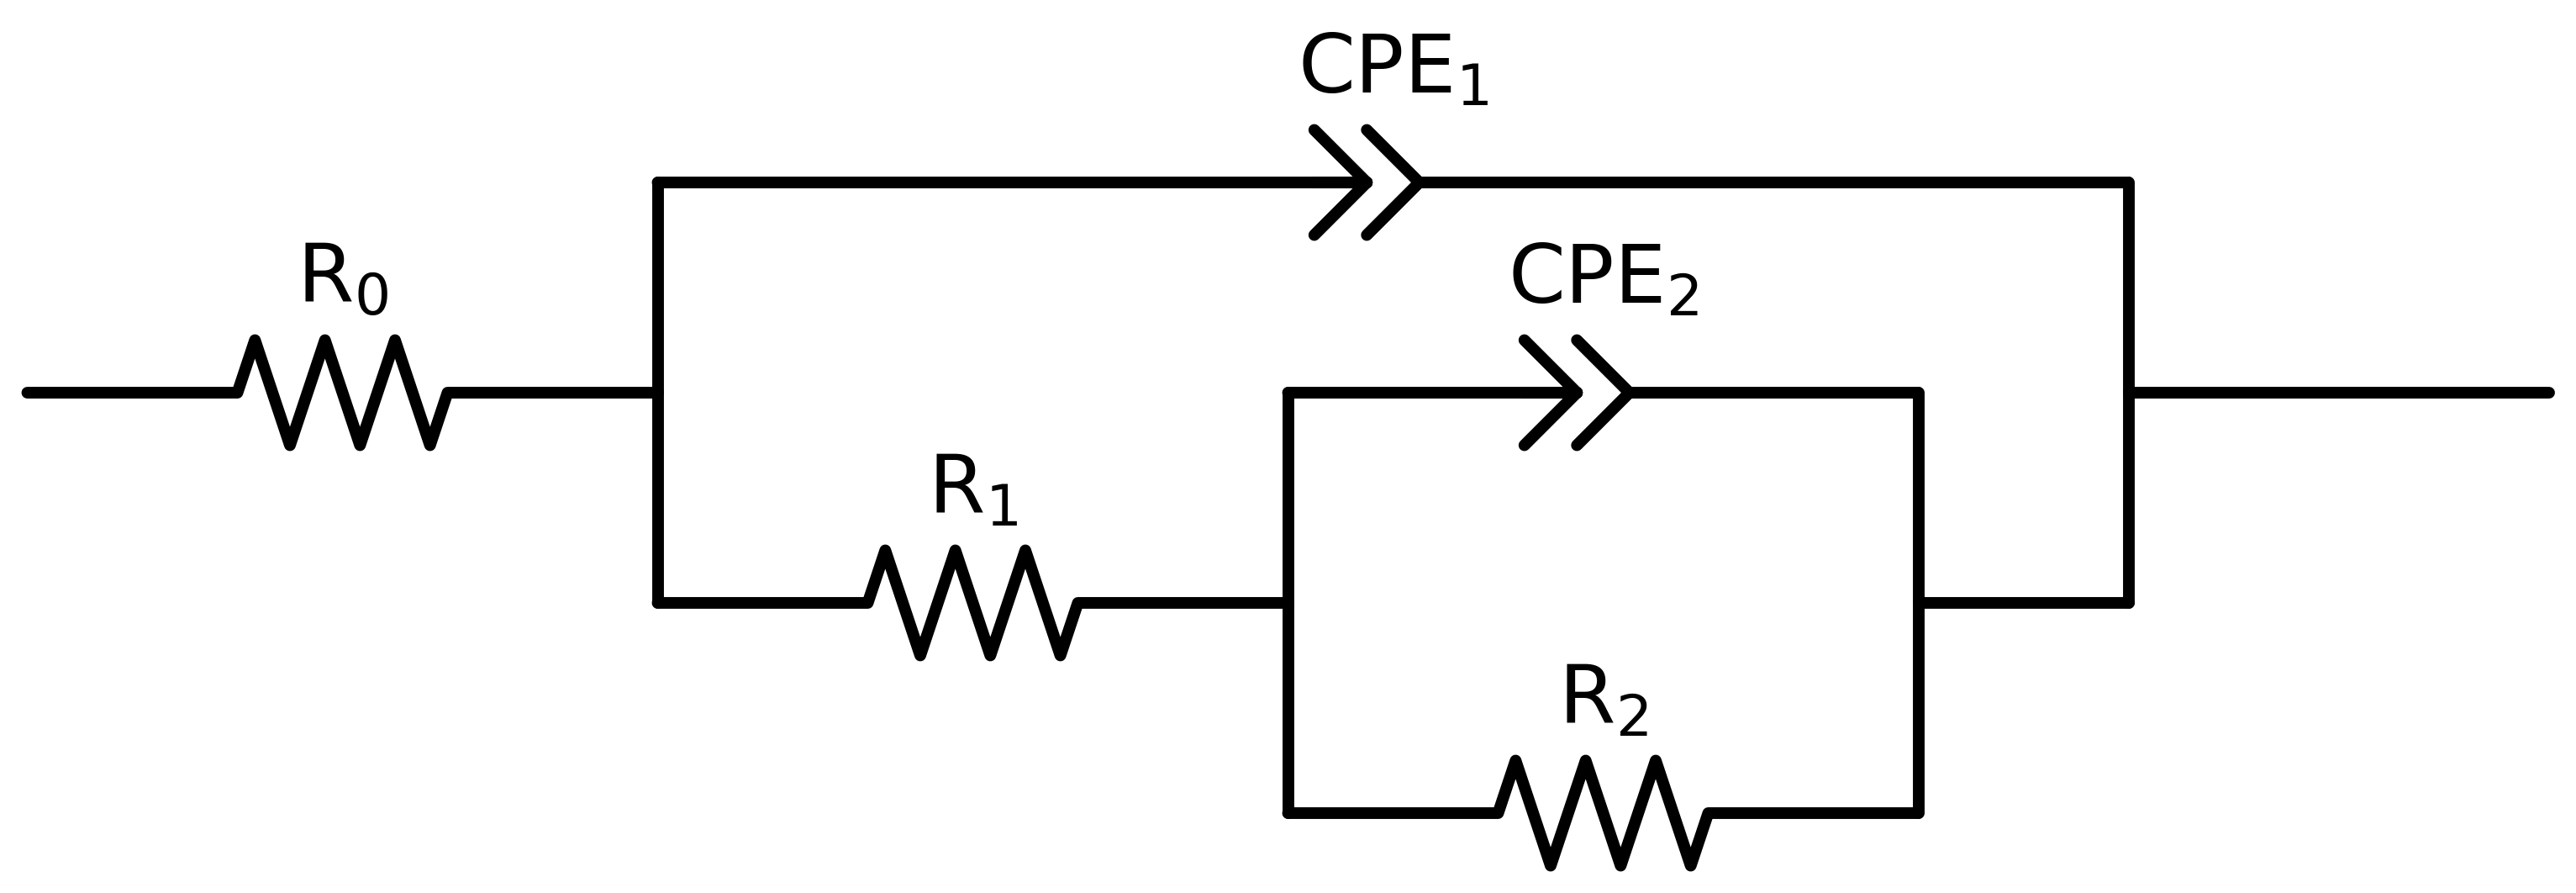
\includegraphics[width=0.45\textwidth]{../../2RC.png}
\end{center}

\renewcommand{\arraystretch}{1.6} 
\begin{table}[h!]
    \centering
    \footnotesize
    \begin{tabular}{|l|c|c|c|c|c|c|}
        \hline
        \textbf{Element} & \textbf{Unit} & \textbf{Bounds} & \textbf{Cauvel\_1\_MBT\_24H} & \textbf{Cauvel\_1\_MBT\_48H} & \textbf{Cauvel\_1\_MBT\_72H} & \textbf{Cauvel\_1\_MBT\_168H} \\ \hline
        $R_{0}$ & $\Omega$ & $[1.0e-03, 1.0e+03]$ & $7.12e+01 \pm 3.3e-01$ & $6.69e+01 \pm 4.2e-01$ & $6.31e+01 \pm 4.1e-01$ & $1.03e+01 \pm 2.3e+01$ \\ \hline
        $R_{1}$ & $\Omega$ & $[1.0e+00, 1.0e+08]$ & $5.79e+05 \pm 5.8e+04$ & $4.03e+02 \pm 5.7e+04$ & $5.79e+05 \pm 5.3e+04$ & $6.24e+01 \pm 2.3e+01$ \\ \hline
        $R_{2}$ & $\Omega$ & $[1.0e+00, 1.0e+08]$ & $3.26e+06 \pm 4.4e+02$ & $1.22e+06 \pm 5.4e+04$ & $1.00e+08 \pm 1.2e-01$ & $2.86e+06 \pm 5.6e+05$ \\ \hline
        $Q_{2}$ & $\Omega$$^{-1}$ sec$^{a}$ & $[1.0e-11, 1.0e-03]$ & $9.37e-06 \pm 3.1e-06$ & $1.58e-06 \pm 2.3e-07$ & $1.46e-05 \pm 5.1e-06$ & $7.96e-06 \pm 3.5e-07$ \\ \hline
        $n_{2}$ & - & $[5.0e-01, 1.0e+00]$ & $5.00e-01 \pm 7.5e-02$ & $5.00e-01 \pm 8.1e-02$ & $5.86e-01 \pm 9.8e-02$ & $8.70e-01 \pm 4.9e-03$ \\ \hline
        $Q_{1}$ & $\Omega$$^{-1}$ sec$^{a}$ & $[1.0e-11, 1.0e-03]$ & $7.50e-06 \pm 5.7e-08$ & $7.11e-06 \pm 4.3e-07$ & $8.43e-06 \pm 7.7e-08$ & $2.46e-06 \pm 3.2e-07$ \\ \hline
        $n_{1}$ & - & $[5.0e-01, 1.0e+00]$ & $8.93e-01 \pm 1.4e-03$ & $8.96e-01 \pm 4.2e-03$ & $8.70e-01 \pm 1.8e-03$ & $5.00e-01 \pm 5.1e-02$ \\ \hline
        \textbf{$\chi^2$} & - & -  & $4.301e-04$ & $7.270e-04$ & $7.742e-04$ & $6.564e-04$ \\ \hline

    \end{tabular}
\end{table}


\newpage
\section*{Analysis Results: 24H}
\begin{center}
    
\includegraphics[width=0.7\textwidth]{plots_Cauvel_1_MBT_24H_2RC.pdf}
    \captionof{figure}{EIS Fit Results for Cauvel\_1\_MBT\_24H}
\end{center}

\newpage
\section*{Analysis Results: 48H}
\begin{center}
    
\includegraphics[width=0.7\textwidth]{plots_Cauvel_1_MBT_48H_2RC.pdf}
    \captionof{figure}{EIS Fit Results for Cauvel\_1\_MBT\_48H}
\end{center}

\newpage
\section*{Analysis Results: 72H}
\begin{center}
    
\includegraphics[width=0.7\textwidth]{plots_Cauvel_1_MBT_72H_2RC.pdf}
    \captionof{figure}{EIS Fit Results for Cauvel\_1\_MBT\_72H}
\end{center}

\newpage
\section*{Analysis Results: 168H}
\begin{center}
    
\includegraphics[width=0.7\textwidth]{plots_Cauvel_1_MBT_168H_2RC.pdf}
    \captionof{figure}{EIS Fit Results for Cauvel\_1\_MBT\_168H}
\end{center}


\end{document}
